\section{मुख्य इलेक्ट्रानिक उपकरण}
	


	\subsection{फोटोडायोड}
	
		फोटोडायोड का उपयोग एक परावर्तक विन्यास में एक डिटेक्टर के रूप में किया जाएगा, जिसमें LED एक छोर से प्रकाश उत्सर्जित करते है और फोटोडायोड विपरीत छोर पर प्रकाश को करंट में परिवर्तित कर रहा है। यह करंट LED प्रकाश की तीव्रता के समानुपाती होगा।
		
		\begin{figure}[ht!]
			\centering
			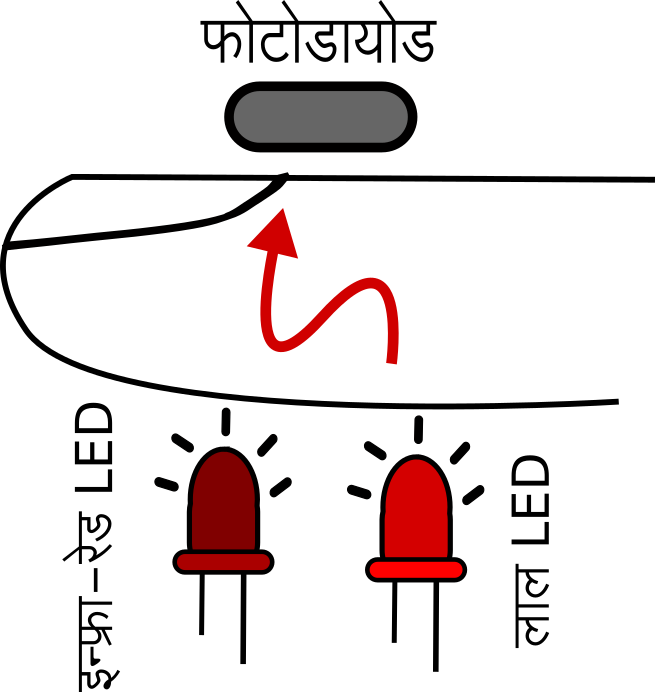
\includegraphics[width=0.3\textwidth]{images/finger_setup_hi.png}
			\caption{चिंतनशील उंगली सेटअप}
		\end{figure}

			इस डिज़ाइन मे फोटोडायोड QSB34CGR का उपयोग किया गया है। देखा जा सकता है, चयनित फोटोडायोड लाल (700nm) और इन्फ्रा-रेड (900nm) क्षेत्रों में संवेदनशील है, इसलिए दोनों स्रोतों को बारी-बारी से प्रकाशित करके विद्युत-धारा तीव्रता मापी जा सकती है।
		\begin{figure}[ht!]
			\centering
			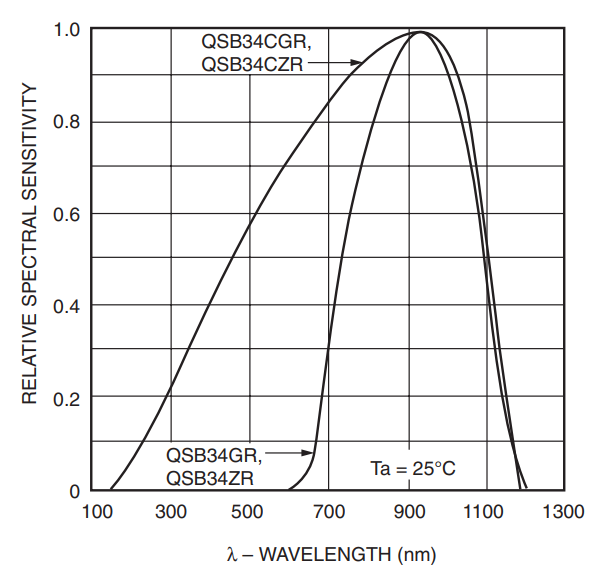
\includegraphics[width=0.6\textwidth]{../common/QSBCGR.png}
			\caption{QSB34CGR स्पैक्ट्रम संवेदनशीलता}
		\end{figure}
	
	\pagebreak
	
	\subsection{माइक्रोकंट्रोलर}
	
		माइक्रोकंट्रोलर($\mu$C) ADC के माध्यम से लाल और इन्फ्रा-रेड प्रवर्धित सिग्नल को पढ़कर SpO\textsubscript{2} की गणना के ऐल्गोरिद्म के लिए जिम्मेदार है। इसके अलावा यह निम्नलिखित कार्य करता है:
		
		\begin{itemize}
			\item गणना की गई SpO\textsubscript{2} और दिल की धड़कन दिखाने के लिए OLED 128x64 डिस्प्ले के साथ इंटरफेस।
			
			\item DACs के साथ इंटरफेस। 
			
		\end{itemize}
		
		इस डिज़ाइन में Atmega4808 का उपयोग किया गया है।
	
	\subsection{दोहरी DAC}
	

		दोहरी डिजिटल से एनालॉग कनवर्टर (DAC) - MCP47FEB02A0 डिजाइन में उपयोग किया गया है।
		
		\begin{itemize}
			
			\item DAC1 की आवश्यकता है ताकि $\mu$C DAC को LED करंट सेट करने के लिए आवश्यक नियंत्रण वोल्टेज उत्पन्न करने का निर्देश दे सके।
			
			\item DAC2 सिगनल से DC को हटाने के लिए डिफ़ैंस एम्पलीफायर चरण के लिए एक इनपुट प्रदान करता है।
		
		\end{itemize}
	
	\subsection{Leds}
		रोशनी के लिए अच्छे led का चयन करना महत्वपूर्ण है, निम्नलिखित कारण अच्छी सिग्नल प्रतिक्रिया सुनिश्चित करते हैं:
				
		\begin{itemize}
			\item कम फैलाव और त्वचा में गहरी प्रवेश के लिए संकीर्ण दृश्य कोण। 
			\item क्लियर lens समकोण पैकेज - ताकि उंगली आराम से led पर बैठ सकें। 
			\item उच्च दीप्तिमान शक्ति। 
		\end{itemize}
		
		मैने 3mm/5mm कि सामान्य leds का उपयोग किया। 5mm कि इन्फ़्ररेड led सर्कुलर क्लियर पैकेज में और 5mm डिफ्यूज्ड पैकेज में लाल led का इस्तेमाल किया डिजाइन मे। इसके कारण R अनुपात सही नहीं हो रहा था। एक स्वस्थ व्यक्ति के रूप में, मुझे R की रीडिंग 0.6 के आसपास मिल रही थी, जबकि यह 0.4 के आसपास होनी चाहिए। इसलिए मुझे ऐल्गोरिद्म को समायोजित करने के लिए स्केलिंग कारक का उपयोग करना पड़ा। इस संबंध में प्रोग्राम कोड में एक कमेंट लिखा गया है। 
		
		Vishay Semiconductor VSMD66694 एक उपयुक्त led हो सकती है आक्सीमीटर के लिये। 
			
		  
	